
% pmk PNAS3 -x prop2_process_local_me 85 95 -m immsb_cgs -c generator7 manufacturing

\begin{subfigure}
     \centering
         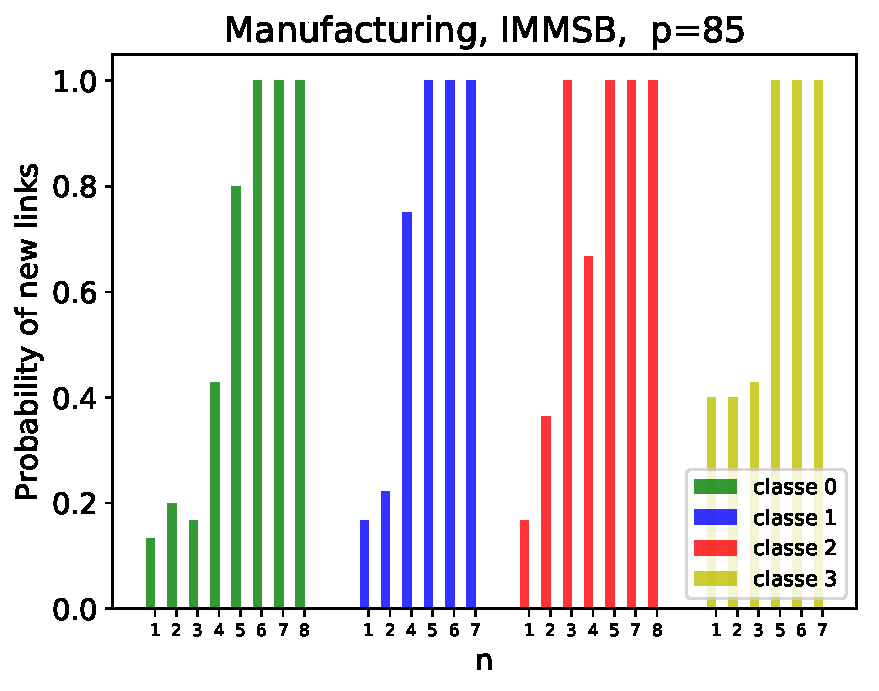
\includegraphics[width=0.45\textwidth]{img/burst/3_prop2_process_local_me__85}
\end{subfigure}
\begin{subfigure}
         \centering
      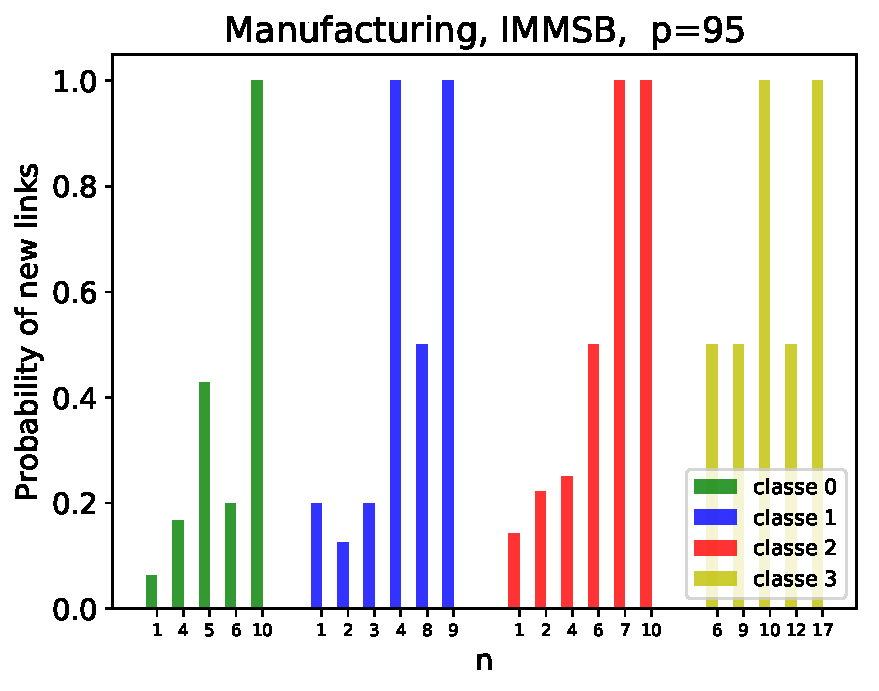
\includegraphics[width=0.45\textwidth]{img/burst/3_prop2_process_local_me__95} 
\end{subfigure}                                                                          
\begin{subfigure}                                                                        
         \centering                                                                      
      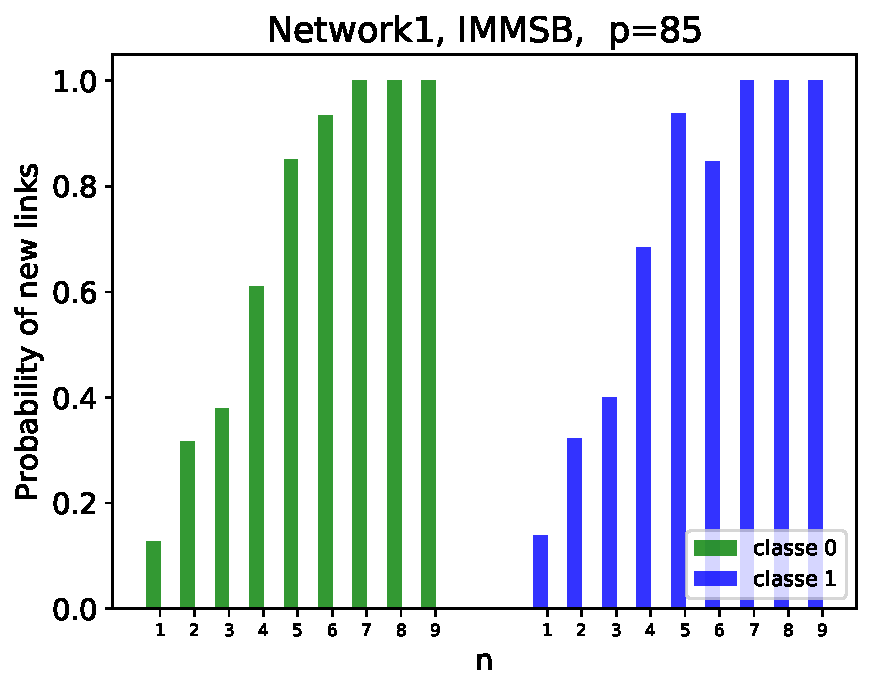
\includegraphics[width=0.45\textwidth]{img/burst/5_prop2_process_local_me__85}
\end{subfigure}                                                                          
\begin{subfigure}                                                                        
         \centering                                                                      
      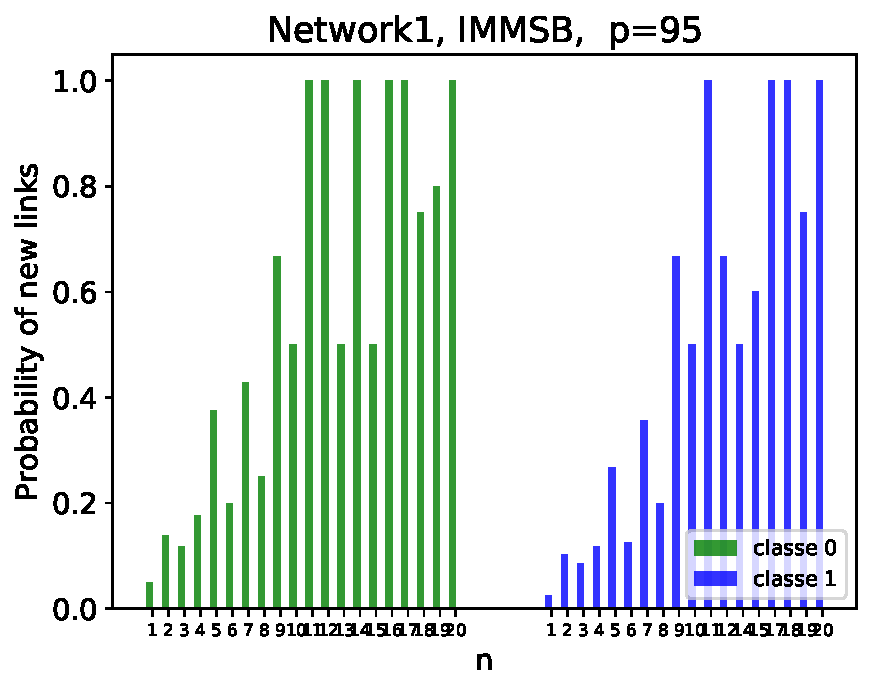
\includegraphics[width=0.45\textwidth]{img/burst/5_prop2_process_local_me__95}
\end{subfigure}                                                                          
\caption{Local burstiness process for IMMSB illustrated by the probability to generate new links for degree at step $p$. The model is fitted with the Manufacturing and networks1 networks for respectively line 1 and 2. First row is for a value of the generating step $p=85\%$ (percentage of the total number of nodes $N$) and $p=95\%$ for the second row . }
\label{fig:burst_immsb}


